%!TEX TS-program = xelatex
%!TEX encoding = UTF-8 Unicode

\documentclass[11pt,tikz,border=1]{standalone}
\usepackage[default,mdseries=Light,bfseries=Medium,path=../fonts]{cjkfonts}
\usetikzlibrary{calc,positioning}

\begin{document}
  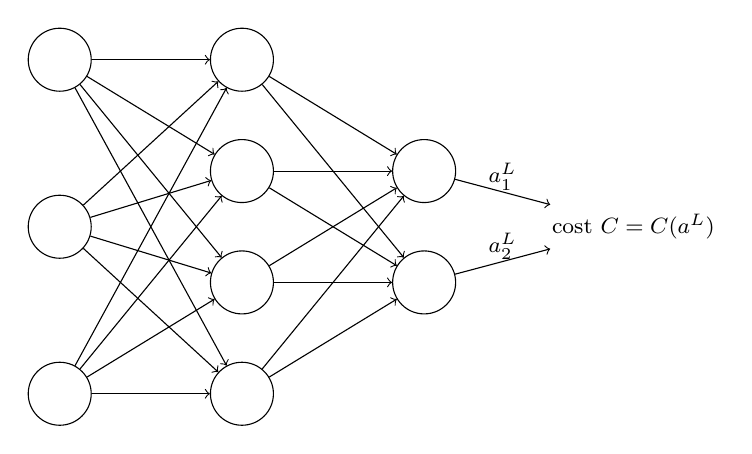
\begin{tikzpicture}[
    neuron/.style={circle,draw,inner sep=0pt,minimum size=8mm},
    font=\footnotesize
    ]
    
    \node(l0) [neuron] {};
    
    \node(m0) [neuron,right=1.5 of l0] {};
    \node(m1) [neuron,above=0.6 of m0] {};
    \node(m2) [neuron,above=0.6 of m1] {};
    \node(m3) [neuron,above=0.6 of m2] {};
    
    \node(l2) [neuron,left=1.5 of m3] {};
    
    \node(r0) [neuron,right=1.5 of m1] {};
    \node(r1) [neuron,right=1.5 of m2] {};
    
    \coordinate (lc) at ($(l0)!0.5!(l2)$);
    \node(l1) at (lc) [neuron] {};
    
    \coordinate (rc) at ($(r0)!0.5!(r1)$);
    \node(eq) [right=1.5 of rc] {cost $C = C(a^L)$};
    
    % connections:
    \foreach \x in {0, 1, 2}
    \foreach \y in {0,...,3}
    \draw[->] (l\x) to (m\y);
    
    \foreach \x in {0,...,3}
    \foreach \y in {0,1}
    \draw[->] (m\x) to (r\y);

    \draw[->] (r0) to node [above,yshift=-1mm] {$a^L_2$} (eq);
    \draw[->] (r1) to node [above,yshift=-1mm] {$a^L_1$} (eq);

  \end{tikzpicture}
\end{document}
